\chapter{Basics on classification}\label{ch:2}

\begin{remark}{Outline}
In this chapter, we introduce classification models from a machine learning perspective. 
First, in Section~\ref{sec:2:classification}, we give a self contained introduction to 
classification, including the most-common algorithms, and the main applications of 
classification models. Then, in Section~\ref{sec:2:measures}, we present the different evaluation 
measures that are normally used for analyzing the performance of classification methods.
\end{remark}

\section{Introduction}
\label{sec:2:classification}

In machine learning, classification refers to the attempt of identifying to which of a set of 
classes a new example belongs, based on learning from examples whose class membership is known. 
The most important point about classification is that for each example only one known class is 
possible, making this a discrete problem. 

A classification task begins with a training set in which the class of a set of examples is known. 
For example, a classification model that predicts credit card fraud is developed by analyzing 
many observed credit transactions over a period of time. The class in this case is a variable which 
indicates for each example whether or not the transaction was or not a fraud. Also, the predictors 
or features, are the transaction attributes like place, amount and time of the transaction.

Then, during the training process, a classification algorithm finds the patterns and relationships 
between the values of the features and the values of the target class. Different algorithms use 
different methods and techniques to estimate the relationships. Afterwards, these relationships are 
summarized in a model that is able to make predictions on new sets of data.

In general, there are two types of classification models: binary and multi-class. In binary 
classification problems the objective is to classify examples between two classes, usually refereed 
as the negative and positive classes. On the other hand, multi-class problems are not bound to two 
classes but instead the algorithms attempt to classify examples among a number of classes. In this 
work we focus on binary classification problems.

Binary classification algorithms are widely used across a variety of domains. For example in the 
medical field, models have been used for making predictions about tumors, probability 
of a disease, probability of selecting the right drug for a particular patient, and estimating the 
probability of relapsing, among others \citep{Herland2014}. In the financial sector, classification 
models have been successfully applied for fraud detection, credit scoring, portfolio management and 
algorithmic trading. Also, in marketing, several models are being currently used for churn modeling, 
customer targeting, behavior prediction and direct marketing \citep{Baesens2014}. Additionally, 
classification algorithms are used in many other emerging applications such as terrorism 
prevention, malware detection, computer security, energy consumption prediction, spam 
classification, and others \citep{Kriegel2007}.

Formally, a binary classification algorithm deals with the problem	of predicting the class $y_i$ 
of a set $\mathcal{S}$ of examples or instances $i$, given their $k$ features \mbox{$\mathbf{x}_i 
\in \mathbb{R}^k$}. The objective is to construct a function $f(\cal{S})$ that makes a prediction 
$c_i$ of the class of each of the $N$ examples using its feature vector $\mathbf{x}_i$, where 
$N=\vert \mathcal{S} \vert$. Moreover, some algorithms allow to not only estimate the prediction, 
but also its confidence, in the form of the probability $\hat p_i$ of belonging to the positive 
class, i.e. $c_i = 1$. The way for going from $\hat p_i$ to $c_i$ is simply by defining a 
probability threshold $t$, and applying the following formula
\begin{equation}\label{eq_pred}
  c_i = 
  \begin{cases}
    \phantom{-}0 \phantom{-} \mbox{if} \phantom{-} \hat p_i \le t\\
    \phantom{-}1 \phantom{-}\mbox{otherwise,}
  \end{cases}
\end{equation}
Usually, $t=\frac{1}{2}$ \citep{Hastie2009}, as an example with probability of being positive 
higher than 50\% is classified as positive, and negative otherwise. If $t \ne \frac{1}{2}$, the 
function that generates the predicted class labels $\mathbf{c}$ is denoted as $f^t$, where 
$\mathbf{c}=\{c_i\}_{i=1}^{N}$.

\begin{figure}
	\centering
	  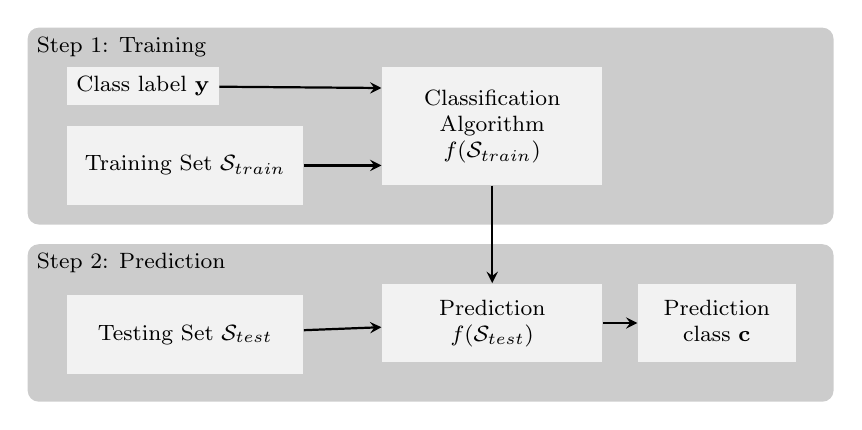
\begin{tikzpicture}[node distance=2cm]
  \tikzstyle{every node}=[font=\footnotesize]
  
  % Main boxes
  \node (step1) [rectangle, rounded corners, anchor=north west, fill=black!20, text width=10cm,
								minimum height=2.5cm] {};
	\node [anchor=north west] at (step1.north west){Step 1: Training};
	\node (step2) [rectangle, rounded corners, anchor=west, fill=black!20, text width=10cm, 
								minimum height=2cm, below of = step1, yshift=-0.5cm] {};
	\node [anchor=north west] at (step2.north west){Step 2: Prediction};
	
	% Training
	\node (label) [rectangle, anchor=north west, fill=black!5,
								yshift=-0.5cm, xshift=0.5cm] {Class label $\bf y $};
	\node (train) [rectangle, anchor=north west, fill=black!5, minimum height=1cm, minimum width=3cm,
								yshift=-1.25cm, xshift=0.5cm] {Training Set $\mathcal{S}_{train} $};
	\node (algo) [rectangle, anchor=north west, fill=black!5, minimum height=1.5cm,
							 minimum width=2.8cm, yshift=-.50cm, xshift=4.5cm] 
							 {\tabular{c} Classification \\ Algorithm  \\	$f(\mathcal{S}_{train}) $
								\endtabular}; 

	%Classification
	\node (test) [rectangle, anchor=north west, fill=black!5, minimum height=1cm, minimum width=3cm,
								yshift=-3.4cm, xshift=0.5cm] {Testing Set $\mathcal{S}_{test} $};
	\node (algo2)[rectangle, anchor=north west, fill=black!5, minimum height=1cm, minimum width=2.8cm,
							 yshift=-3.25cm, xshift=4.5cm] 
							 {\tabular{c} Prediction \\	$f(\mathcal{S}_{test}) $\endtabular};
	\node (pred) [rectangle, anchor=north west, fill=black!5, minimum height=1cm,
							yshift=-3.25cm, xshift=7.75cm] {\tabular{c} Prediction \\ class $\bf c$	\endtabular};
	
	% Arrows
	\node (label_temp) [rectangle, anchor=north west, yshift=-0.65cm, xshift=4.5cm] {};
	\draw[thick,->,>=stealth] (label) to (label_temp);
	\node (train_temp) [rectangle, anchor=north west,minimum height=1cm, minimum width=3cm,
								yshift=-1.25cm, xshift=4.5cm] {};
	\draw[thick,->,>=stealth] (train) to (train_temp);
	\draw[thick,->,>=stealth] (algo) to (algo2);
	\draw[thick,->,>=stealth] (test) to (algo2);
	\draw[thick,->,>=stealth] (algo2) to (pred);
  \end{tikzpicture}
 
  \caption{Classification process}
  \label{fig:2:1}
\end{figure}

In \figurename{ \ref{fig:2:1}}, the process of training and prediction in a classification 
algorithm are summarized. First, during the training phase, using a training set 
$\mathcal{S}_{train}$, an algorithm is trained to predict $\mathbf{y}$, where
$\mathbf{y}=\{y_i\}_{i=1}^{N}$. Then the algorithm is used to estimate the classes 
$\mathbf{c}$ of a set of testing examples $\mathcal{S}_{test}$.

\begin{figure}[!t]
\centering
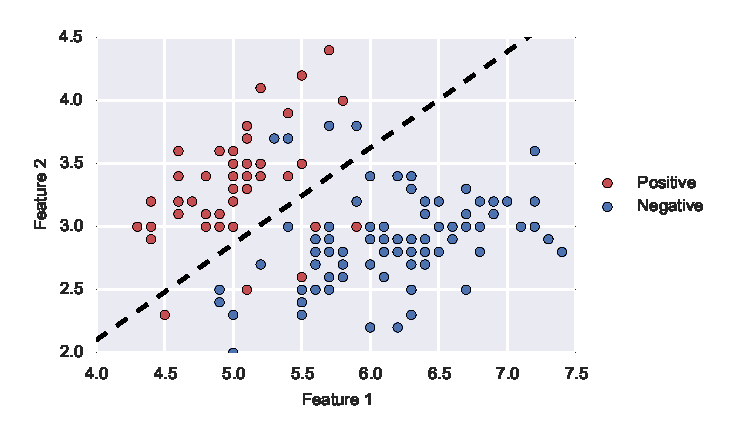
\includegraphics{ch2_fig1b}
\caption{Example of a classification algorithm. Using a set of examples from two classes, a 
	classification algorithm is learned in order to separate between the positives and the negatives. 
}
\label{fig:2:2}
\end{figure} 

There exists several algorithms that can be used for classification tasks. In general a 
classification algorithm is learned with the objective of finding patterns that separate between 
the different classes \citep{Hastie2009}. In order to clarify this intuition, in \figurename{ 
\ref{fig:2:2}} an example of a classification algorithm is shown. Let us suppose a set of 
examples, where the red points represent the positive examples and the blue ones the negative 
examples. The objective of a classifier is to find the best way to separate between the positive and 
negative examples. Then, the output of a classifier learned using the set of training examples is 
shown as the dashed black line. It is observed that this classifier is able to separate almost all 
the examples using a linear classifier. However, not all examples are correctly classified. In 
particular, there are four negative examples that were predicted as positive, and five positive 
examples that were predicted as negative. In the next section, we present the standard methods for 
evaluating the performance of a classification algorithm.


\section{Performance evaluation measures}
\label{sec:2:measures}

When evaluating the performance of a classification algorithm, the first thing to do is to check 
the number of examples that were misclassified. Since the true class of the examples 
is known. Therefore, evaluating the error of a model is as simple as counting the number of times 
an example is misclassified divided by the number of examples
\begin{equation}\label{eqn:ch2:error}
Err(f({\cal S})) = 1 -\frac{1}{N}  \sum_{i=1}^N \mathbf{1}_{y_i}(c_i),
\end{equation}
where $\mathbf{1}_q(z)$ is an indicator function that is calculated as:
\begin{equation}
   \mathbf{1}_q(z) = 
  \begin{cases}
    \phantom{-}1 \phantom{-} \mbox{if} \phantom{-} z \in q\\
    \phantom{-}0 \phantom{-} \mbox{if} \phantom{-} z \notin q.
  \end{cases}
\end{equation}
Moreover the accuracy is defined as the percentage of times the algorithm 
made the correct prediction
\begin{equation}\label{eqn:2:accuracy}
Acc(f({\cal S})) = 1- Err(f({\cal S})).
\end{equation}

However, just knowing these statistics is not enough to make decisions, as in many applications 
it is important to know where the errors are coming from. In particular, the misclassified examples 
may belong only to one class, which may give interesting insights about the problem. A way to 
observe the different errors is by looking at the confusion matrix, as shown in 
\mbox{\tablename{~\ref{tab:2:1}}}. Afterwards, using the cost matrix several statistics are 
extracted. In particular:
  \begin{flalign}
    &Recall = \frac{TP}{TP+FN} &\\
    &Precision = \frac{TP}{TP+FP}& \\
    &F_1Score = 2\frac{Precision \cdot Recall}{Precision + Recall}&
  \end{flalign}
  
	\begin{table}[!t]
		\centering
		\footnotesize
    \begin{tabular}{c|c|c}
      \multicolumn{3}{c}{}\\
			\multicolumn{1}{c|}{}  & Actual Positive& Actual Negative \\
			\multicolumn{1}{c|}{} & $y_i=1$& $y_i=0$ \\
			\hline
			Predicted Positive 		& \multirow{ 2}{*}{True Positive ($TP$)} & \multirow{ 
			2}{*}{False Positive ($FP$)} \\
			$c_i=1$ & &\\
			\hline
			Predicted Negative  	& \multirow{ 2}{*}{False Negative ($FN$)} & \multirow{ 
			2}{*}{True Negative ($TN$)} \\
			$c_i=0$ & &\\
		\end{tabular}
		\caption{Classification confusion matrix}
		\label{tab:2:1}
  \end{table}  
 
 \newpage
  As an illustrative example, the different statistics are calculated for the example presented 
  in Section~\ref{sec:2:classification}. First, the confusion matrix is calculated as 
  follows:
  \begin{center}
    \footnotesize
  \begin{tabular}{c|c|c}
    \multicolumn{1}{c|}{}  & Actual Positive& Actual Negative \\
    \multicolumn{1}{c|}{} & $y=1$& $y=0$ \\
    \hline
    Predicted Positive    & \multirow{ 2}{*}{36} & \multirow{ 
    2}{*}{4} \\
    $c=1$ & &\\
    \hline
    Predicted Negative    & \multirow{ 2}{*}{5} & \multirow{ 
    2}{*}{68} \\
    $c=0$ & &\\
  \end{tabular}
  \end{center}
  Then using the confusion matrix, the different statistics are calculated as: Error = 
11.11\%, Recall = 87.8\%, Precision = 90\% and $F_1Score$ = 88.8\%.
	
There are, however, several instances that are misclassified, that is because the simple linear 
classifier that was used in this example may not be good enough to separate between the positive 
and negative classes. In order to make a comparison, using the same example, a new 
algorithm is learned. This time the algorithm made the correct prediction more often as shown in 
\figurename{ \ref{fig:2:3}}. Afterwards, the confusion matrix is calculated as follows:

\begin{figure}[t!]
  \centering
  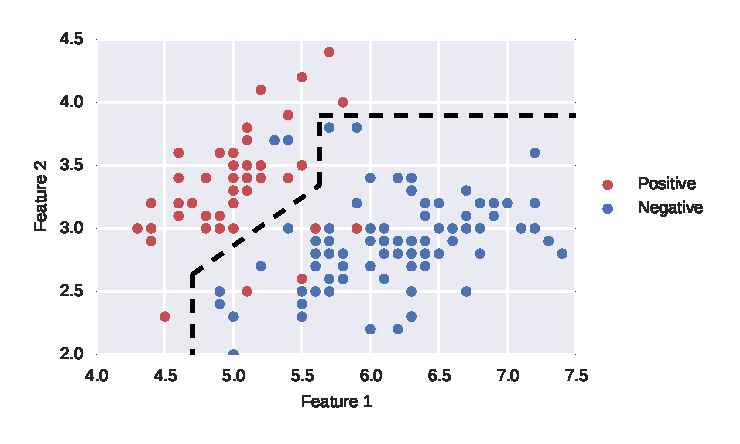
\includegraphics{ch2_fig2}
  \caption{Example of a classification algorithm. Using a set of examples from two classes, a 
  classification algorithm is learned in order to separate between the positives and the negatives. 
}
  \label{fig:2:3}
\end{figure}

\begin{center}
		\footnotesize
    \begin{tabular}{c|c|c}
			\multicolumn{1}{c|}{}  & Actual Positive& Actual Negative \\
			\multicolumn{1}{c|}{} & $y=1$& $y=0$ \\
			\hline
			Predicted Positive 		& \multirow{ 2}{*}{37} & \multirow{ 
			2}{*}{2} \\
			$c=1$ & &\\
			\hline
			Predicted Negative  	& \multirow{ 2}{*}{4} & \multirow{ 
			2}{*}{70} \\
			$c=0$ & &\\
		\end{tabular}
\end{center}
Then the different statistics are calculated as: Error = 5.3\%, Recall = 90.2\%, Precision = 
94.9\% and $F_1Score$ = 92.5\%.
It is observed that in this case the FP are reduced more than the FN, this leads to a higher 
increase in precision  than in recall. There is not a single rule regarding which one is more 
important than the other, it depends on the applications. For example in applications with a high 
false negative cost such as failing to identify a tumor in a medical exam, the recall should be the 
priority, even if that implies having a significant number of false positives. On the other hand, 
In applications such as spam detection, predicting a normal email as spam it may have a large 
impact on the customer, therefore, in this example is better to allow some false negatives and 
focus on the false positives.

It is not always straightforward  to define the right tradeoff between false positives 
and false negatives. The best approximation to solve that, is to focus on the actual costs incurred 
by the different decisions. This is usually solved using cost-sensitive classification methods. 

\subsection{Brier score}
\label{sec:2:brier}

Traditional evaluation measures of binary classification problems, such as Accuracy and 
$F_1Score$, provide a way to analyze the performance of a model. However, when using the classifier 
output as a basis for decision making, there is a need of a measure that takes into account not 
only the misclassification of a classifier predicted class $c$, but also the quality of the 
estimated probabilities $\mathbf{\hat p}$ \citep{cohen2004}. The most appropriate  is the Brier 
score \citep{brier1950}. The Brier score belongs to the class of so-called proper scores which are 
used in evaluating the subjective probability assessment of the prediction \citep{DeGroot1983}. The 
Brier score is the average squared difference between the estimated probability and the true class 
label. It is defined as:
\begin{equation}
  BS(f(\mathcal{S})) = \frac{1}{N} \sum_{i=1}^{N} (\hat p_i - y_i)^2.
\end{equation}

The main justification of this score is based on decision theoretic considerations, in the sense 
that, a forecaster should pay a price proportional to the confidence with which it asserts its 
decision.


\subsection*{}
